%
% einleitung.tex -- Beispiel-File für die Einleitung
%
% (c) 2020 Prof Dr Andreas Müller, Hochschule Rapperswil
%
% !TEX root = ../../paper.tex
% !TEX encoding = UTF-8
%
\section{Geschichte\label{geostrophisch:section:geschichte}}
\kopfrechts{Geschichte}

Die Anfänge der numerischen Wettervorhersage gehen auf den britischen Mathematiker und Physiker \textbf{Lewis Fry Richardson} (1881–1953) zurück.  
In seinem Werk \textit{Weather Prediction by Numerical Process} (1922) formulierte Richardson als Erster die Idee, eine numerische Wettervorhersage durch das explizite Lösen eines physikalisch fundierten Gleichungssystems zu bestimmen.  
Damit legte er den theoretischen Grundstein für die moderne Wettermodellierung.
Für diese Erste Vorhersage von 6 Stunden brauchte er etwa 6 Wochen Zeit für die Berechnungen.
Zudem wich diese auch noch weit von der Realität ab.
Warum das so war und warum seine Arbeit trotzdem so wichtig für heutige Wettervorhersagen ist, darauf gehen wir in den folgenden Kapiteln ein. 

\begin{figure}[h]
	\centering
	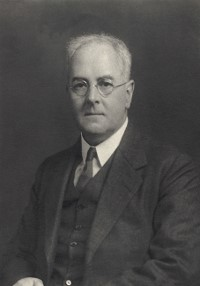
\includegraphics{Portrait_Richardson.jpg}
	\caption{Portraitfoto von Richardson}
	\label{bild:portraitRichi}
\end{figure}

Siehe ~\ref{bild:portraitRichi} das ist ein Portrait Foto von Richardson.

\begin{itemize}
	\item \textbf{Bewegungsgleichungen:} Horizontale und vertikale Impulsbilanz
	\item \textbf{Kontinuitätsgleichung:} Erhaltung der Masse
	\item \textbf{Energiegleichung:} Thermodynamische Prozesse
	\item \textbf{Zustandsgleichung:} Zusammenhang zwischen Druck, Temperatur und Dichte
\end{itemize}






